\documentclass[11pt]{article}
\usepackage{latexsym}
\usepackage{amsmath}
\usepackage{amssymb}
\usepackage{amsthm}
\usepackage{epsfig}
\usepackage[tight]{subfigure}
\usepackage{hyperref}

\usepackage{amsmath}

\DeclareMathOperator*{\minimize}{min}
\DeclareMathOperator*{\maximize}{max}

\usepackage{algorithm}
 %on linux you may need to run sudo apt-get install texlive-full to install algorithm.sys
\usepackage{algorithmic}

\usepackage{verbatim}

\newcommand{\handout}[5]{
  \noindent
  \begin{center}
  \framebox{
    \vbox{
      \hbox to 5.78in { {#1} \hfill #2 }
      \vspace{4mm}
      \hbox to 5.78in { {\Large \hfill #5  \hfill} }
      \vspace{2mm}
      \hbox to 5.78in { {\em #3 \hfill #4} }
    }
  }
  \end{center}
  \vspace*{4mm}
}

\newcommand{\lecture}[5]{\handout{#1}{#2}{#3}{#4}{#5}}
\newcommand{\collision}[0]{\mathrm{collision}}
\newcommand{\nocollision}[0]{\overline{\collision}}

\newcommand*{\QED}{\hfill\ensuremath{\square}}

\newtheorem{theorem}{Theorem}
\newtheorem{corollary}[theorem]{Corollary}
\newtheorem{lemma}[theorem]{Lemma}
\newtheorem{observation}[theorem]{Observation}
\newtheorem{proposition}[theorem]{Proposition}
\newtheorem{definition}[theorem]{Definition}
\newtheorem{claim}[theorem]{Claim}
\newtheorem{fact}[theorem]{Fact}
\newtheorem{assumption}[theorem]{Assumption}
\newtheorem{note}[theorem]{Note}

% 1-inch margins, from fullpage.sty by H.Partl, Version 2, Dec. 15, 1988.
\topmargin 0pt
\advance \topmargin by -\headheight
\advance \topmargin by -\headsep
\textheight 8.9in
\oddsidemargin 0pt
\evensidemargin \oddsidemargin
\marginparwidth 0.5in
\textwidth 6.5in

\parindent 0in
\parskip 1.5ex
%\renewcommand{\baselinestretch}{1.25}

\begin{document}

\lecture{Statistical Techniques in Robotics (16-831, S22)}{Lecture \#09
  (Wednesday, February 16)}{Lecturer: Kris Kitani}{Scribes: Young Woo Kim, Daphne Chen}{Online Gradient Descent}

\section{Review}
In the previous lecture we covered Online Mirror Descent (OMD). This is an extension to the content about convex optimization, including the Follow the Regularized Leader (FTRL) algorithm. FTRL can be interpreted as a form of OMD, thus in this lecture we will cover how OMD and OGD are connected to various online learning and optimization problems. 

% In the last lectures, on the topic of Prediction with Expert Advice (PWEA), we had analyzed three main algorithms: (1) Greedy, (2) Halving, and (3) Randomized Greedy. In this lecture, we will introduce and analyze two more algorithms for the PWEA problem, namely: the Weighted Majority Algorithm (WMA) and the Randomized Weighted Majority Algorithm (RWMA). For a quick high level takeaway, we note that the Weighted Majority Algorithm (WMA) has a bounded regret, while the RWMA is our first no regret algorithm. This lecture, after the review section, will derive these results. In the next two subsections, we first recap the problem of prediction with expert advice and a few definitions to help us along the way in deriving those results.

%This section serves as a review of the previous lecture and any other context required to frame the content of the current lecture. 

%You may format the scribes in any way you like, aside from changing font style, size and page format. Please use subsections and paragraphs to increase the readability of your notes.

%Length requirement 1-2 pages.

\subsection{Follow the Regularized Leader (FTRL)}
Follow the Regularized Leader \cite{mcmahan2011ftrl}, similarly to OMD, is a class of online optimization algorithms; however, it uses a regularization function instead of a mirror function in order to stabilize the loss function. In general, the algorithm uses the following steps:

\begin{algorithm}[H]
\caption{Follow the Regularized Leader (FTRL)}
\label{algo:ftrl}
\begin{algorithmic}[1]
\STATE \textsc{\textbf{function}} FTRL(Convex set $S$)
\FOR{$t=1,\;\cdots,\;T$}
\STATE $\textbf{w}^{(t)} = argmin_{\textbf{w}} \Sigma_{i=1}^{t-1} f^{(i)}(\textbf{w}) + \psi(\textbf{w})$ \hfill $\triangleright$ prediction rule with regularization
\STATE \textsc{Receive} ($f^{(t)} : S \rightarrow \mathbb{R}$) \hfill $\triangleright$ one step loss
\ENDFOR
\end{algorithmic}
\end{algorithm}

Where the loss function is linear, and uses quadratic regularization, as follows:

\begin{align}
    \psi(w) = \frac{1}{2\eta} ||w||_2^2 \label{eq:quadreg}
\end{align}

\begin{align}
    f^{(t)} = w \cdot z^{(t)} \label{eq:linearloss}
\end{align}

Where Equation \ref{eq:quadreg} is the quadratic regularization and \ref{eq:linearloss} is the linear loss.

The regret bound of the FTRL algorithm is given by the equation below:

\begin{align}
    R^{(T)}(\textbf{u}) \leq BL \sqrt{2T} \label{eq:FTRLregret}
\end{align}

% TODO proof of regret bound

In summary, the FTRL algorithm displays the following properties:

\begin{enumerate}
    \item \textbf{\textit{Varying regret:}} regret varies depending on the choice of loss function
    \item \textbf{\textit{Regularized:}} FTRL uses regularization to ensure stability and no-regret property
\end{enumerate}


\subsection{Online Mirror Descent (OMD)}
We previously covered two forms of online optimization – FTRL and OMD. Online Mirror Descent uses a mirror function. FTRL and OMD can be interpreted as each other, but provide a different set of tools for online learning and regret analysis. OMD acts as a mathematical framework for connecting concepts between online learning and convex optimization.

The basis for the OMD algorithm are the steps shown below:

\begin{algorithm}[H]
\caption{Online Mirror Descent (OMD)}
\label{algo:omd}
\begin{algorithmic}[1]
\STATE \textsc{\textbf{function}} OMD(Convex set $S$, $g : \mathbb{R}^D \rightarrow S$)
\FOR{$t=1,\;\cdots,\;T$}
\STATE \textsc{Receive} ($f^{(t)} : S \rightarrow \mathbb{R}$) \hfill $\triangleright$ mirror function
\STATE $\theta^{(t+1)} = {\theta}^{(t)} - \eta z^{(t)}, z^{(t)} \in \partial f^{(t)}(w^{(t)})$
\STATE $\textbf{w}^{(t+1)} = g(\theta^{(t+1)})$ \hfill $\triangleright$ prediction rule 
\ENDFOR
\end{algorithmic}
\end{algorithm}

The general idea for OMD is that it can adapt to the size of the gradient. The tradeoff, however, is that the algorithm may perform poorly when it diverges from the optimal parameters, as may happen when there is a significant change in the data during the online learning process, a problem which FTRL mitigates. 

% https://www.timvanerven.nl/blog/ftrl-vs-omd/


\section{Summary}
\subsection{Gradient Descent}
\normalfont
Gradient descent is the standard method we use to minimize differentiable convex functions. It can be used to minimize nonconvex functions as well, but it may converge to a local minimum instead of a guaranteed global minimum, as it would for convex functions. The lecture discusses three perspectives to understanding gradient descent.

\subsubsection{Geometric Perspective}
% We can include a visual like the one on slide 6 to take up space if we want
The geometric perspective of gradient is the intuitive idea of taking the gradient of a function and stepping in the direction opposite of it. Over many steps, we can imagine sufficient steps would approach the minimum of the function. This intuition is described in Algorithm 1


\begin{algorithm}[H]
\caption{Gradient Descent (GD)}
\label{algo:gd}
\begin{algorithmic}[1]
\STATE $\textbf{w}^{(0)} \leftarrow \textbf{0}$ \hfill $\triangleright$ Weight initialization
\FOR{$t=1,\;\cdots,\;T$}
\STATE \textsc{Compute} ($\nabla f(\textbf{w}^{(t-1))}$) \hfill $\triangleright$ Compute Gradient
\STATE $\textbf{w}^{(t)} = \textbf{w}^{(t-1)} - \eta \nabla f(\textbf{w}^{(t-1)})$ \hfill $\triangleright$
Step opposite gradient direction
\ENDFOR
\end{algorithmic}
\end{algorithm}

Algorithm 1 provides the skeleton of gradient descent, but it is more intuitive than rigorous. For a function $f:\mathbb{R}^N \rightarrow \mathbb{R}$, the gradient is the vector $\nabla f(\textbf{w}) = \{ \frac{\partial f(\textbf{w})}{w_1}, \cdots, \frac{\partial f(\textbf{w})}{w_N} \}$.

\subsubsection{Linear Approximation with Regularization}
The second perspective on gradient descent recognizes that we can take a convex function we want to minimize, compute its first order Taylor series approximation at $\textbf{w}$ and use it to lower bound the function at another point $\textbf{u}$.  
$$f(\textbf{u}) \geq f(\textbf{w}) + \langle \textbf{u} - \textbf{w}, \nabla f(\textbf{w}) \rangle$$
%Include a visual 
Suppose we try to minimize this linear function directly; the solution would be at negative infinity, though this is obviously untrue of the original convex function. We must account for the fact that linear approximations are only accurate near the point $\textbf{w}$ and must therefore be constrained by a regularizer that encourages closeness to $\textbf{w}$. For an L2 regularizing term, the final objective function is as follows:

$$\textbf{w}^{(t+1)} = \text{argmin}_w \frac{1}{2}||\textbf{w} - \textbf{w}^{(t)}||^2 + \eta \Big( f(w^{(t)}) + \langle w - w^{(t)}, \nabla f(w^{(t)})\rangle \Big) $$

\subsubsection{Isometric Quadratic Approximation}
The third perspective uses the second order approximation of the convex function f: 
$$f(u) \approx f(w) + (u+w)^T \nabla f(w) + \frac{1}{2}(u-w)^T \nabla^2f(w)(u-w)$$
The second order gradient, however, can be expensive to compute, so we replace it with an identity matrix and introduce a scaling parameter to further approximate the convex function as such:

$$f(u) \approx f(w) + (u+w)^T \nabla f(w) + \frac{1}{2\eta}(u-w)^T I(u-w)$$
We can now see the second order term simplifies into the L2 regularization term from the linear approximation perspective.
$$\textbf{w}^{(t+1)} = \text{argmin}_w \frac{1}{2}||\textbf{w} - \textbf{w}^{(t)}||^2 + \eta \Big( f(w^{(t)}) + \langle w - w^{(t)}, \nabla f(w^{(t)})\rangle \Big) $$

To solve this equation, we take the first order derivative of the expression we want the argmin of set it to zero. Doing so yields the familiar update equation for w, which we have seen in online perceptron, weighted majority, and follow the regularized leader.
$$w = w^{(t)} - \eta \nabla f(w^{(t)})$$

\subsection{Stochastic Gradient Descent}
Generally, it is expensive to compute the gradient of the loss function f in the update equation because f is usually a sum over the losses of many data points. We can speed it up by performing the updates in batches, so the entire data set does not need to be evaluated for each update. To achieve maximal efficiency, we can set the batch size to 1 and update after each training example. This example is chosen at random, or stochastically. The new estimated gradient at each iteration will no longer equal the original gradient direction, but the expected gradient will. This algorithm is known as stochastic gradient descent and similar convergence bounds as gradient descent.

\begin{algorithm}[H]
\caption{Stochastic Gradient Descent (SGD)}
\label{algo:sgd}
\begin{algorithmic}[1]
\STATE $\textbf{w}^{(1)} \leftarrow \textbf{0}$ \hfill $\triangleright$ Weight initialization
\STATE $\eta > 0$ \hfill $\triangleright$ Set learning rate
\FOR{$t=1,\;\cdots,\;T$}
\STATE $z \sim \mathcal{D}$ \hfill $\triangleright$ Mini-batch or Single Sample
\STATE $\textbf{v}^{(t)} = \nabla f_z(\textbf{w}^{(t-1))}$) \hfill $\triangleright$ Compute Faster Gradient
\STATE $\textbf{w}^{(t)} = \textbf{w}^{(t-1)} - \eta \nabla \textbf{v}^{(t)}$ \hfill $\triangleright$
Step opposite gradient direction
\ENDFOR
\end{algorithmic}
\end{algorithm}

\subsection{OGD/SGD as a Special Case of Mirror Descent (OMD)}
Recall the Online Mirror Descent algorithm from Section 1.2. We will now observe how online gradient descent can be represented in the mirror descent framework. OMD updates parameters in the primal space by updating parameters in the dual space and mapping it to the primal parameters using a mirror function. OMD with the quadratic regularization function $\psi(w) = \frac{1}{2\eta} ||w||^2_2 $ and linear loss function $f(w) = \langle w, \theta \rangle$ results in the following prediction rule:
\begin{align*}
w^{(1+t)} &= \arg \min\limits_{w} \langle w, -\theta^{(t+1)} \rangle  + \frac{1}{2\eta} ||w||^2_2 \\
 &= \arg \min\limits_{w} \langle w, -\theta^{(t+1)} \rangle  + \frac{1}{2\eta} \sum\limits_n w^2_n
\end{align*}
We can now describe the loss function $\mathbb{L}$ as follows:
$$\mathbb{L} = \langle w, -\theta \rangle + \frac{1}{2\eta} \sum\limits_n w^2_n$$
$$\frac{\partial \mathbb{L}}{\partial w_n} = -\theta_n + \frac{1}{2\eta} 2w_n = 0$$
$$w_n = \eta\theta_n$$
This shows that the optimal parameter for $w_n$ is $\eta \theta_n$, and that our mirror function for OGD is the trivial projection $g(\theta) = \eta\theta$. Note that this results in an update rule similar to the one in the perceptron algorithm. To summarize, online gradient descent is online mirror descent with a linear loss and quadratic regularization.


\subsection{OGD Regret Analysis}

In order to derive the regret bound for OGD, we will define the following equation:

\begin{align}
    R_{OGD} \leq DG\sqrt{T}
\end{align}

Where $D = max || \textbf{u} ||_2, u \in S$ (assumption on the magnitude of the primal parameter) and $G = max || \textbf{z} ||_2, z \in \partial f(\textbf{w})$ (assumption on the magnitidue of the sub-gradient, related to dual parameter). We also need to recall the regularization function and the convex conjugate for OGD. 

Let us assume that we use the L2 norm for the regularizer. Then the convex conjugate is also L2 norm, or:

\begin{align}
    \psi({w}) = \frac{1}{2} ||w||_2^2 \\
    \psi^*({\theta}) = \frac{1}{2} ||\theta||_2^2
\end{align}

From here, we can start from the general regret bound analysis for OMD to derive the regret bound for OGD.

\begin{align}
    R(u) &\leq \psi(u) - \psi(w^{(1)}) + \sum_{t=1}^T D_{\psi^*} (\theta^{(t+1)} || \theta^{(t)}) \label{eq:omd_regret_1} \\
    &= \psi(u) - \psi(w^{(1)}) + \sum_{t=1}^T \psi^* (\theta^{(t+1)}) - \psi^*(\theta^{(t)}) - \nabla \psi^* (\theta^{(t)})(\theta^{(t+1)} - \theta^{(t)}) \label{eq:omd_regret_2}
\end{align}

Using the Bregman divergence under the L2 norm in Equations \ref{eq:omd_regret_1} and \ref{eq:omd_regret_2}.

\begin{align}
    &= \frac{1}{2\eta}||u||_2^2 - \frac{1}{2\eta}||w^{(1)}||_2^2 + \sum_{t=1}^T \frac{1}{2\eta}||\theta^{(t+1)}||_2^2 - \frac{1}{2\eta}||\theta^{(t)}||_2^2 - \nabla \frac{1}{2\eta}||\theta^{(t)}||_2^2 (\theta^{(t+1)} - \theta^{(t)}) \label{eq:omd_regret_3} \\
    &= \frac{1}{2\eta}||u||_2^2 - \frac{1}{2\eta}||w^{(1)}||_2^2 + \sum_{t=1}^T \frac{1}{2\eta}||\theta^{(t+1)}||_2^2 - \frac{1}{2\eta}||\theta^{(t)}||_2^2 - \frac{1}{\eta}\theta^{(t)} (\theta^{(t+1)} - \theta^{(t)}) \label{eq:omd_regret_4}
\end{align}

In Step \ref{eq:omd_regret_3} computing the gradient, and in Step \ref{eq:omd_regret_4} completing the square.

\begin{align}
    &= \frac{1}{2\eta}||u||_2^2 - \frac{1}{2\eta}||w^{(1)}||_2^2 + \sum_{t=1}^T \frac{1}{2\eta}||\theta^{(t+1)} - \theta^{(t)}||_2^2  \label{eq:omd_regret_5} \\
    &= \frac{1}{2\eta}||u||_2^2 - \frac{1}{2\eta}||w^{(1)}||_2^2 + \sum_{t=1}^T \frac{1}{2\eta}||\theta^{(t)} - \eta z^{(t)} - \theta^{(t)}||_2^2  \label{eq:omd_regret_6} \\
    &= \frac{1}{2\eta}||u||_2^2 - \frac{1}{2\eta}||w^{(1)}||_2^2 + \sum_{t=1}^T \frac{1}{2\eta}|| -\eta z^{(t)} ||_2^2  \label{eq:omd_regret_7}
\end{align}

Where we plug in the definition of dual parameter in Step \ref{eq:omd_regret_5} and then subtract terms, finally removing the always positive term in Step \ref{eq:omd_regret_7}.

Lastly, this results in the following bound:

\begin{align}
    &\leq \frac{1}{2\eta}||u||_2^2 + \sum_{t=1}^T \frac{\eta}{2}|| z^{(t)} ||_2^2  \label{eq:omd_regret_8}
\end{align}

Thus we have derived the regret bound for OGD.

In order to derive the optimal step size $\eta$, assuming that $T$ is known, we can take the derivative:

\begin{align}
    \frac{d}{d\eta} \{\frac{1}{\eta} D^2 + \frac{\eta}{2} G^2T \} = 0 \rightarrow \eta = \frac{D}{G\sqrt{T}}
\end{align}

And subsequently plug back in to the equation for OGD regret bound, in order to get the result:

\begin{align}
    R_{OGD}(U) &\leq \frac{D^2}{2\eta} + \frac{\eta}{2} T^2G \\
    &= DG\sqrt{T}
\end{align}

\subsection{Online Normalized Exponentiated Gradient Descent (ONEGD)}

We have noted that different choices of regularization can result in different mirror functions and different algorithms. Another such algorithm is normalized exponentiated gradient descent. Instead of the quadratic regularization term from OGD, we now use the negative entropy regularization and the linear loss function. 
$$\psi(\textbf{w}) = \sum\limits_{k=1}^{K} w_k \log w_k, \textbf{w} \in \mathbb{S}^K$$
$$f(w) = \langle w, \theta \rangle $$
This yields the following prediction rule:
$$w^{(t+1)} = \arg \min\limits_{w \in \mathbb{S}^K} \langle w, -\theta^{(t+1)} \rangle + \sum\limits_{k=1}^K w_k \log w_k $$
We then add the simplex constraint to this objective:
$$w^{(t+1)} = \arg \min\limits_{w \in \mathbb{S}^K} \langle w, -\theta^{(t+1)} \rangle + \sum\limits_{k=1}^K w_k \log w_k + \lambda \Big( 1 - \sum_{k} w_k\Big)$$
$$\mathbb{L} = \langle w, -\theta^{(t+1)} + \frac{1}{\eta} \sum\limits_{k=1}^K w_k \log w_k  + \lambda \big( 1-\sum_k w_k \big)$$
By solving for the minimum of this loss function, we get the following w and mirror function
$$w_n = \frac{\exp (\eta \theta_k}{\exp(1- \eta \lambda)}$$
$$g(\theta) = \frac{\exp (\eta \theta}{\sum\limits_{n'}\exp(\eta \theta_{n'})}$$

\begin{algorithm}[H]
\caption{Online Normalized Exponentiated Gradient Descent (ONEGD)}
\label{algo:onegd}
\begin{algorithmic}[1]
\STATE $\textbf{function} \textsc{Online Norm-Exp-GD}(\eta)$
\FOR{$t=1,\;\cdots,\;T$}
\STATE $\theta^{(t+1)} = \theta^{(t)} - \eta z^{(t)}, z^{(t)} \in \partial f^{(t)}(w^{(t)})$  \hfill $\triangleright$ Dual parameter update
\STATE $\textbf{w}^{(t+1)} \propto - \exp \big( \eta\theta^{(t+1)} \big)$ \hfill $\triangleright$
Mirror projection
\ENDFOR
\end{algorithmic}
\end{algorithm}


\section{Conclusion}

In this lecture we covered the topic of Online Gradient Descent. We learned about how this relates to the prior lectures on Online Mirror Descent and other forms of online learning problems. Delving into the topic of Online Gradient Descent, we covered the necessary background on gradient descent from three different perspectives, including the geometric perspective, using linear approximation with regularization, and isometric quadratic approximation. Subsequently, we algorithmically studied stochastic gradient descent, noting the similar convergence bounds between GD and SGD. Relating this back to earlier lectures, we analyzed how OGD and SGD can be described as special cases of OMD. We concluded by performing a regret bound analysis for OGD, followed by one last method, online normalized exponentiated gradient descent.

%\section*{References}
%Include your references here. Please cite any resources you found useful.	
%Populate the refs.bib file or list your references manually. Be consistent in formatting!
{
\bibliography{refs}
\bibliographystyle{abbrv}
}

\section{Appendix}
%This section provides any relevant background material that was not covered in the lectures, but was found to be useful for understanding the material. 
%For example, derivations, theory underlying techniques employed, etc. 

%Additionally, this section can summarizes applications or extensions of these techniques found in the literature. 

\subsection{Duality}

This section will cover mathematical concepts that enable us to analyze OMD, namely conjugate functions and the Bregman divergence.

\subsubsection{Conjugate Functions}

A convex conjugate function, also known as a Fenchel conjugate, is a generalization of the Legendre transform. For the purpose of this course, we assume a smooth convex function, but the Legendre generalization can also be applied to non-smooth and non-convex functions.

The base formula for a convex conjugate function is as follows in Equation \ref{eq:conjugate}:

\begin{align}
    \psi^*(\theta) = \max_w (\langle \theta, w \rangle - \psi(w)) \label{eq:conjugate}
\end{align}

Next, we will analyze the geometry of the conjugate function. If we use intercept-slope parametrization (e.g. $\{\psi(w), w\}$, purple curve in below figure) with the function-value parametrization (e.g. $\{b(\theta), \theta \}$, green lines in below figure), as shown in the figure below (referenced from the \href{https://www.dropbox.com/sh/j3cnwem4wo1u3bx/AADlFGyy7quBUsXrnQ3hda6La?dl=0&preview=L8+OMD-Duality.pdf}{class notes}), then we can get the dual curve (or duality) that consists of a curve $C$ and a set of lines tangent to $C$. 

\begin{center}
    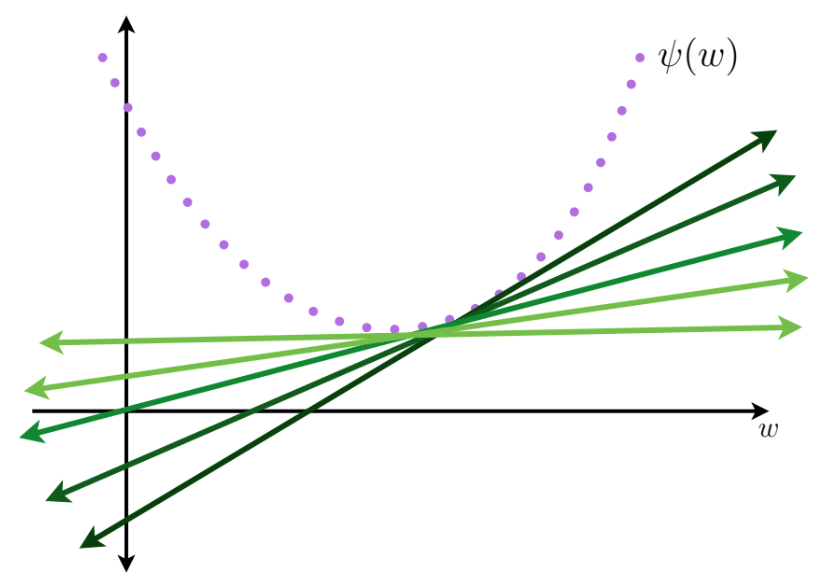
\includegraphics[width=10cm]{duality.png}
\end{center}

Given the function $\psi(w)$, the value $\theta$ is the derivative of $\psi$ at $w = w^*$, thus the equation for the tangent line is $y = \langle \theta, w \rangle - b$. Using this formula, the "slope" or vertical distance between the y-intercept $b$ and the tangent point is given as $\langle \theta, w \rangle$, or $\psi(w^*) + b$ using the curve in the figure. Thus the equation is updated to the following:

\begin{align}
    \langle \theta, w^* \rangle = \psi(w^*) + b(\theta) \\
    -b(\theta) = -\langle \theta, w^*(\theta) \rangle + \psi(w^*(\theta))
\end{align}

Using the geometry described above, we can now show how this holds for the conjugate function. The maximum distance between two functions, given in Equation \ref{eq:conjugate}, is equal to the intercept of the tangent line, shown visually in the below figure (referenced from the \href{https://www.dropbox.com/sh/j3cnwem4wo1u3bx/AADlFGyy7quBUsXrnQ3hda6La?dl=0&preview=L8+OMD-Duality.pdf}{class notes}). 

\begin{center}
    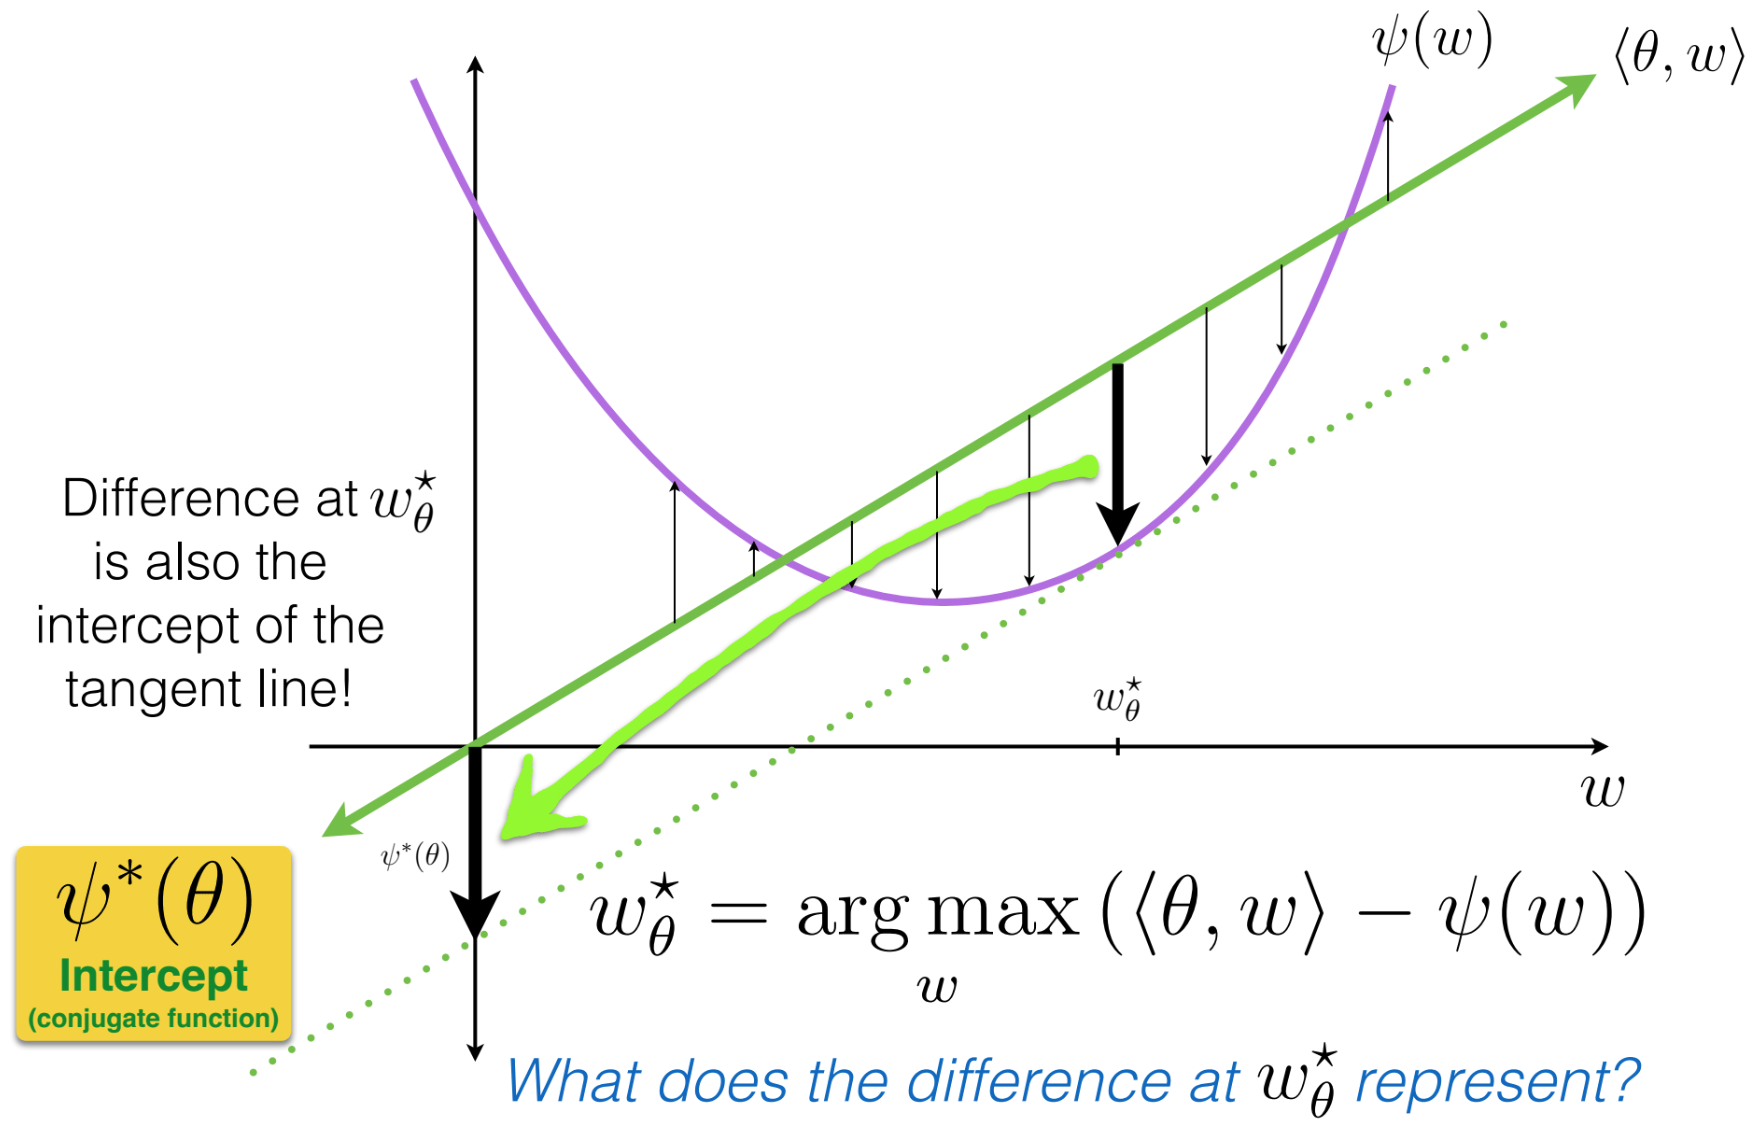
\includegraphics[width=10cm]{tangent-conjugate.png}
\end{center}

The derivative of the convex conjugate function is given as:

\begin{align}
    \nabla_\theta \psi^*(\theta) = arg\max_w (\langle \theta, w \rangle - \psi(w)) \label{eq:derivative_conjugate}
\end{align}

The Fenchel-Young inequality is:

\begin{align}
    \psi^*(\theta) \geq (\langle \theta, w \rangle - \psi(w)) \label{eq:fenchel_young}
\end{align}


\subsubsection{Bregman Divergence}

The Bregman Divergence is represented in Equation \ref{eq:bregman}:

\begin{align}
    D_\psi(w||u) = \psi(w) - \psi(u) - \nabla\psi(u)^T(w-u)  \label{eq:bregman}
\end{align}

Where the distance $D$ is defined between two points with a proximity function $\psi$. In the context of OMD, this means the regularization function.

% The geometry of the Bregman Divergence  TODO 


\end{document} % Done!


